% !TEX program = xelatex
\documentclass{article}

%% ---- Set up paper margin ---- %%
%\usepackage[a4paper,top=1in,bottom=1in,left=1in,right=1in]{geometry}

% use multiple languages
%% ---- allow CJK usage ---- %%
\usepackage[CJKspace]{xeCJK} % this should be called before Polyglossia
\setCJKmainfont{Noto Serif CJK TC}
\setCJKsansfont{Noto Sans CJK TC}
\setCJKmonofont{Noto Sans Mono CJK TC}
% \setCJKmainfont{Noto Serif JP}
% \setCJKsansfont{Noto Sans JP}
% \setCJKmonofont{Noto Sans Mono CJK JP}

%% ---- ตั้งค่าให้ตัดคำภาษาไทย ---- %%
\XeTeXlinebreaklocale "th"
\XeTeXlinebreakskip = 0pt plus 0pt % เพิ่มความกว้างเว้นวรรคให้ความยาวแต่ละบรรทัดเท่ากัน

%% ---- font settings ---- %%
\usepackage{fontspec}
\defaultfontfeatures{Mapping=tex-text} % map LaTeX formating, e.g., ``'', to match the current font
% To change the main font, uncomment one of the below command.
% \setmainfont{TeX Gyre Termes} % Free Times
% \setsansfont{TeX Gyre Heros} % Free Helvetica
% \setmonofont{TeX Gyre Cursor} % Free Courier
\newfontfamily{\thaifont}[Scale=MatchUppercase,Mapping=textext]{Laksaman} % ตั้งฟอนต์หลักภาษาไทย
\newenvironment{thailang}{\thaifont}{} % create environment for Thai language
\usepackage[Latin,Thai]{ucharclasses} % ตั้งค่าให้ใช้ "thailang" environment เฉพาะ string ที่เป็น Unicode ภาษาไทย
\setTransitionTo{Thai}{\begin{thailang}}
\setTransitionFrom{Thai}{\end{thailang}}

%% ---- spacing between lines ---- %%
\usepackage{setspace}
% \singlespacing % default setting
% \onehalfspacing % recommend using this for Thai language

%% ---- using alphabatic language ---- %%
\usepackage{polyglossia}
\setdefaultlanguage{english} % it is preferrable to set English as the main language, since the numeric system is compatible with most LaTeX features such as 'enumerate' and so on
\setotherlanguages{thai}

\AtBeginDocument\captionsthai % allow captions to be in Thai


%% ---- math packages ---- %%
\usepackage{amsmath}
\usepackage{amssymb}
\usepackage{bm} % same functionality as \mathbf{} but for greek letters
\usepackage{diffcoeff}
\usepackage{physics}
\usepackage{mathdots}
\numberwithin{equation}{section} % equation numbers are formatted as <#Section>.<#eq in the section>

%% ---- define math environment ---- %%
\usepackage{amsthm}
\newtheorem{definition}{Definition}[section]
% \newtheorem{definition}{Definition}
\newtheorem{proposition}[definition]{Proposition}
\newtheorem{theorem}[definition]{Theorem}
\newtheorem{corollary}{Corollary}[definition]
\newtheorem{remark}{Remark}[definition]
\newtheorem{lemma}[definition]{Lemma}
\newtheorem{problem}[definition]{Problem}
% \newtheorem*{problem}{Problem}

%% ---- hyperref settings ---- %%
\usepackage{hyperref}
\usepackage{url}
\usepackage{cite}
\usepackage{xcolor}
\hypersetup{
    colorlinks,
    linkcolor={red!50!black},
    citecolor={green!50!black},
    urlcolor={blue!80!black}
    }

%% ---- misc. packages ---- %%
\usepackage{enumitem} % allow customizing list environments: enumerate, itemize and description.
\usepackage{mhchem} % use chemistry notation
\usepackage{lipsum}
\usepackage{metalogo} % for extended LaTeX logo such as XeTeX
\usepackage{subcaption} % allowing subfigure environment
% \usepackage[section]{placeins} % ensure floats do not go into the next section and allow the use of \FloatBarrier
\usepackage{graphicx} % allow cropping and rotating images
\usepackage{caption}
\usepackage{float} % allow the use of [H] for positioning of tables and figures
\usepackage{tikz-cd}
\restylefloat{table}

%% ---- title, authors, and dates ---- %%
\usepackage{authblk}
\title{A schematic model of passive urine concentrating mechanism}
\author[1]{Chanoknun Sintavanuruk}
% \affil[1]{Department of Physiology, Faculty of Medicine Siriraj Hospital, Mahidol University}
% \author[2,3]{XXXX XXXX}
% \affil[2]{Department of XXXX, XXXX University}
% \affil[3]{Department of XXXX, XXXX University}
\date{\today}

\begin{document}
\sloppy % ช่วยตัดคำภาษาไทย
\maketitle

\section{Introduction and research log}

Concentration gradient in the renal medullary interstitium is responsible for concentrating urine.
It is well-understood that the active reabsorption of NaCl from the thick ascending tubules, together with the counter-current multiplication, establish this concentration gradient in the outer medulla.
For the inner medulla, where there is no such an active transport, it is the passive reabsorption of NaCl and urea that take over; this is the widely accepted passive mechanism hypothesis of urine concentration.
To have the passive mechanism working, we need to have relatively high tubular concentration of NaCl at the turning of loops of Henle, and of urea in the collecting tubules.
A common explanation is that the net water and NaCl reabsorption preceding the inner medulla collecting tubules concentrate the urea enough that it diffuses out in the inner medulla.
This in turn increases osmolality in the interstitium that drives the water reabsorption from the thin descending limbs, concentrating NaCl in the process.
The aim of this document is to provide a clean picture of the passive mechanism through a relatively simple model.

\subsection{Research log}

\begin{proof}[July 20, 2023.]
    With certain simplifying assumptions, we derive a schematic model of inner medulla with a central core configuration and containing only two solute species: salt and urea (Section \S2).
    We show that the model can be written as a system of 4 ordinary differential equations.
    Our numerical simulations identify factors that contribute to the passive mechanism: the salt input from the outer medulla (which reflects the ratio between short- and long-loop nephrons), and the solute permeability.
    The roles of urea and long-loop nephron are briefly discussed in Section \S3.
\end{proof}

\begin{proof}[July 26, 2023.]
    After meeting with Alan Weinstein, we learned that yielding a negative result from the schematic model would be very meaningful; it would strongly signal that we need a new idea to tackle this problem, e.g., \textit{salt dump} by red blood cells (suggested by Alan Weinstein).
    Indeed, the derivation of this model is in the favor of the classical explanation of the passive mechanism, which makes this model a `\textit{best case scenario}' model.
    We need to determine the extent of concentrating capability to which this model can generate.
    The factors that we need to consider are the size of urea permeable region (realistically, this is the lower $1/3$ of the collect tubule) and the parameter space of the solute permeability (our numerical method only yield convergence for the small values).

    Suppose that this is true, then we can also use this model to investigate the salt dump by adding a source term in the equation for the central core.
\end{proof}

\begin{proof}[August 4, 2023.]
    After introducing salt dump, we discover another steady state solution which collides with the previously known solution as we increase the rate of salt dump, resembling a saddle-node bifurcation.
    It turns out that this steady state also exists and went unnoticed when there is no salt dump.
    However, we can only compute this for a small region of $\gamma_s,\gamma_u\in (1.0,1.2)$.
    We need a dynamic simulation to understand what is going on.
    Namely, we want to know the stability of the steady states and the dynamical behavior in the unknown region of parameter space.
\end{proof}

\begin{proof}[August 16, 2023]
    We go back to the balance equations for the 5 solutes and 4 water flows.
    The time derivative terms are reintroduced for the 5 solutes.
    After numerical experiment, we found that the original steady state is stable while the other is not.
    Moreover, there is yet another stable steady state above the unstable one, thus we have a bistability when $\gamma_s=\gamma_u=1.2$.
    Interestingly, when we increase $\gamma_u,\gamma_s$ beyond $\sim 1.3$ the osmolarity at $x=1$ seems to grow exponentially fast, possibly reaching singularity.
    Apparently, this is the behavior after the unstable and the original steady states merge.
    But what happens to the new stable steady state?
\end{proof}


\section{Model derivation}

% The key idea behind the construction of this model is to reproduce the qualitative explanation of the passive mechanism that passive urea reabsorption from the collecting tubules drives descending tubules water and ascending tubules NaCl reabsorption.
% Any assumption we made in the process will be in the favor of this explanation.

We consider a steady-state model of the inner medulla.
We use $k$ to identify the compartments in the inner medulla: the central core ($k=0$), descending tubules ($k=\mathrm{D}$), ascending tubules ($k=\mathrm{A}$), and the collecting tubules ($k=\mathrm{C}$).
Each compartment is described in a 1-dimensional spatial domain $x\in (0,1)$ where $x=0$ represents the outer-inner medullary junction, and $x=1$ the renal papilla.

We denote by $s_k$, $u_k$ and $q_k$, as a function of $x$, the salt and urea concentration and the axial water flow in the compartment $k$ respectively.
For simplicity, we will assume that the urea content in the descending tubule and the salt content in the collecting tubule are negligible, i.e., $u_\mathrm{D}=s_\mathrm{C}\equiv 0$.
Thus, there are total of 9 unknowns in the model: the water flow $q_\mathrm{D},q_\mathrm{A},q_\mathrm{C},q_0$ and the solute concentrations $s_\mathrm{D},s_\mathrm{A},s_0,u_\mathrm{C},u_0$.

We assume that the transmural water fluxes are allowed only for the descending tubules and the collecting tubules into the interstitium, and these are formally described as $w_\mathrm{D}:=\zeta_\mathrm{D}(2s_0+u_0-2s_\mathrm{D})$ and $w_\mathrm{C}:=\zeta_\mathrm{C}(2s_0+u_0 - u_\mathrm{C})$ where $\zeta_k>0$ is the water permeability, i.e., the fluxes are proportional to the osmolarity differences.
Note that the osmolarity of salt is twice the concentration.
By mass balance, we require that
\begin{align}
    \frac{dq_\mathrm{D}}{dx} &= -\zeta_\mathrm{D}\left( 2s_0+u_0 - 2s_\mathrm{D} \right) = -w_\mathrm{D},\label{eq:q_D_eq}\\
    \frac{dq_\mathrm{A}}{dx} &= 0,\label{eq:q_A_eq}\\
    \frac{dq_\mathrm{C}}{dx} &= -\zeta_\mathrm{C}\left( 2s_0+u_0 - u_\mathrm{C} \right) = -w_\mathrm{C},\label{eq:q_C_eq}\\
    \frac{dq_0}{dx} &= w_\mathrm{D}+w_\mathrm{C}.\label{eq:q_0_eq}
\end{align}
These equations are accompanied by 4 boundary conditions:
\begin{equation}\label{eq:q_bdry}
    q_\mathrm{D}(0) = \frac{2S}{C},\quad q_\mathrm{A}(1) = -q_\mathrm{D}(1),\quad q_\mathrm{C}(0) = \frac{U}{C},\quad q(1) = 0.
\end{equation}
Here, we assume that the initial osmolarity at the beginning (outer-inner medullary junction) of the descending and the collecting tubule is $C$, and the initial salt and urea flow are $S$ and $U$ respectively.
The second equality represents the turning of the loop of Henle, and we have no-flux boundary at the papillary interstitium for the last equality.

Similarly, we only allow passive transmural fluxes of salt from the ascending tubule and of urea from the collecting tubules.
The fluxes are given by $\gamma_s(s_\mathrm{A} - s_0)$ and $\gamma_u(u_\mathrm{C} - u_0)$ respectively, where $\gamma_s$ is the ascending tubule salt permeability and $\gamma_u$ is the collecting tubule urea permeability.
Further, we assume that the axial solute flows are purely advective, i.e., the salt and urea flows are $s_kq_k$ and $u_kq_k$.
As earlier, we have balance equations for salt and urea:
\begin{align}
    \frac{d}{dx}(s_\mathrm{D}q_\mathrm{D}) &= 0,\label{eq:s_D_eq}\\
    \frac{d}{dx}(s_\mathrm{A}q_\mathrm{A}) &= -\gamma_s(s_\mathrm{A} - s_0),\label{eq:s_A_eq}\\
    \frac{d}{dx}(s_\mathrm{0}q_\mathrm{0}) &= \gamma_s(s_\mathrm{A} - s_0),\label{eq:s_0_eq}\\
    \frac{d}{dx}(u_\mathrm{C}q_\mathrm{C}) &= -\gamma_u(u_\mathrm{C} - u_0),\label{eq:u_C_eq}\\
    \frac{d}{dx}(u_\mathrm{0}q_\mathrm{0}) &= \gamma_u(u_\mathrm{C} - u_0).\label{eq:u_0_eq}
\end{align}
The equations (\ref{eq:s_D_eq}) and (\ref{eq:u_C_eq}) are subject to boundary conditions:
\begin{equation}\label{eq:solute_bdry}
    2s_\mathrm{D}(0) = u_\mathrm{C}(0) = C,
\end{equation}
    which describe the initial osmolarity of the descending and the collecting tubules.

Since we have nine ODEs, we need 3 more boundary conditions.
These are obtained by the conservation of water, salt and urea:
\begin{align}
    \frac{2S}{C}+q_0(0)+q_\mathrm{A}+\frac{U}{C} &= q_\mathrm{C}(1),\label{eq:w_consv}\\
    S+q_\mathrm{A}(0)s_\mathrm{A}(0)+s_0(0)q_0(0) &= 0,\label{eq:s_consv}\\
    U+u_0(0)q_0(0) &= u_\mathrm{C}(1)q_\mathrm{C}(1).\label{eq:u_consv}
\end{align}



The system of nine ordinary differential equations we just obtained can be simplified even further.
First, we can turn the differential equation describing the salt concentration in the descending tubules (\ref{eq:s_D_eq}) into an algebraic equation.
With the boundary condition $s_\mathrm{D}(0)q_\mathrm{D}(0) = S$, integrating (\ref{eq:s_D_eq}) yields
\begin{equation}\label{eq:s_D}
    s_\mathrm{D} = \frac{S}{q_\mathrm{D}}.
\end{equation}

For the ascending tubule, in place of the water balance equation (\ref{eq:q_A_eq}), we simply have $q_A$ being constant.
With the salt conservation (\ref{eq:s_consv}) and (\ref{eq:s_D}), summing (\ref{eq:s_A_eq}) and (\ref{eq:s_0_eq}) and taking integral gives
\begin{equation}\label{eq:s}
    S+s_\mathrm{A}q_\mathrm{A}+s_0q_0 = s_\mathrm{D}q_\mathrm{D}+s_\mathrm{A}q_\mathrm{A}+s_0q_0 = 0.
\end{equation}
Note the second equality of (\ref{eq:s}) and the boundary condition $q_\mathrm{A}(1) = -q_\mathrm{D}(1)$ imply that $s_\mathrm{D}(1) = s_\mathrm{A}(1)$.
Consequently, by integrating (\ref{eq:q_A_eq}) we obtain an equation for $q_A$:
\begin{equation}\label{eq:q_A}
    % q_\mathrm{A} = -q_\mathrm{D}(1) = -\frac{S}{s_\mathrm{D}(1)} = -\frac{S}{s_\mathrm{A}(1)}.
    q_\mathrm{A} = -q_\mathrm{D}(1).
\end{equation}
% The salt concentration $s_\mathrm{A}$ is still governed by the same equation (\ref{eq:s_A_eq}), with a boundary condition (\ref{eq:w_consv}).

Now, we solve the equations for the central core (\ref{eq:q_0_eq}), (\ref{eq:s_0_eq}), and (\ref{eq:u_0_eq}).
Similarly to how we obtain (\ref{eq:s}), using the urea conservation (\ref{eq:u_consv}), we have by summing (\ref{eq:u_C_eq}) and (\ref{eq:u_0_eq}) and integrating
\begin{equation}\label{eq:u}
    u_\mathrm{C}q_\mathrm{C}+u_0q_0 = u_\mathrm{C}(1)q_\mathrm{C}(1).
\end{equation}
From the first equality of (\ref{eq:s}) and (\ref{eq:q_A}), we can write
\begin{equation}\label{eq:q_0}
    % q_0 =-\frac{s_\mathrm{A}q_\mathrm{A}+S}{s_0} = -\frac{S}{s_0}\left( 1-\frac{s_\mathrm{A}}{s_\mathrm{A}(1)}  \right).
    q_0 =\frac{s_\mathrm{A}q_\mathrm{D}(1)-S}{s_0}.
\end{equation}
Substituting $q_0$ into (\ref{eq:u}) yields
\begin{equation}\label{eq:su1}
    % s_0\left( u_\mathrm{C}(1)q_\mathrm{C}(1) - u_\mathrm{C}q_\mathrm{C} \right) + u_0S\left( 1-  \frac{s_\mathrm{A}}{s_\mathrm{A}(1)} \right) = 0.
    s_0\left( u_\mathrm{C}(1)q_\mathrm{C}(1) - u_\mathrm{C}q_\mathrm{C} \right) + u_0\left( s_\mathrm{A}q_\mathrm{D}(1) - S \right) = 0.
\end{equation}
We can do the same for the water conservation as well.
Summing (\ref{eq:q_D_eq}), (\ref{eq:q_A_eq}), (\ref{eq:q_C_eq}) and (\ref{eq:q_0_eq}) and integrating, we have $q_\mathrm{D}+q_\mathrm{A}+q_\mathrm{C}+q_0 = q_\mathrm{C}(1)$.
By substituting $q_\mathrm{A}$, $q_0$ from (\ref{eq:q_A}) and (\ref{eq:q_0}), we obtain
\begin{equation}\label{eq:su2}
    q_\mathrm{D}-q_\mathrm{D}(1)+q_\mathrm{C}+\frac{s_\mathrm{A}q_\mathrm{D}(1) - S}{s_0} = q_\mathrm{C}(1).
\end{equation}
We can now solve (\ref{eq:su1}) and (\ref{eq:su2}) for $s_0$ and $u_0$ in terms of $\mathrm{s}_A$, $u_\mathrm{C}$ and $q_\mathrm{C}$:
\begin{equation}\label{eq:su}
    s_0 = \frac{S-s_\mathrm{A}q_\mathrm{D}(1)}{q_\mathrm{D} - q_\mathrm{D}(1)+q_\mathrm{C} - q_\mathrm{C}(1)},\quad u_0 = \frac{u_\mathrm{C}q_\mathrm{C} - u_\mathrm{C}(1)q_\mathrm{C}(1)}{q_\mathrm{D} - q_\mathrm{D}(1)+q_\mathrm{C} - q_\mathrm{C}(1)}.
\end{equation}

With all the 5 unknowns solved, the problem is reduced to a system of ODEs with 4 differential equations:
\begin{align}
    \frac{dq_\mathrm{D}}{dx} &= -\zeta_\mathrm{D}\left( 2s_0+u_0-\frac{2S}{q_\mathrm{D}} \right) \label{eq:sys_q_D}\\
    \frac{ds_\mathrm{A}}{dx} &= -\frac{\gamma_s}{q_\mathrm{A}}(s_\mathrm{A} - s_0),\label{eq:sys_s}\\
    \frac{dq_\mathrm{C}}{dx} &= -\zeta_\mathrm{C}(2s_0+u_0-u_\mathrm{C}),\label{eq:sys_q_C}\\
    \frac{du_\mathrm{C}}{dx} &= \frac{1}{q_\mathrm{C}}\left(\zeta_\mathrm{C}u_\mathrm{C}(2 s_0+u_0 - u_\mathrm{C})- \gamma_u(u_\mathrm{C} - u_0)\right),\label{eq:sys_u}
\end{align}
    with boundary conditions
\begin{equation}\label{eq:sys_bdry}
    % \begin{gathered}
        % s_\mathrm{A}(0) = s_0(0) + s_\mathrm{A}(1)\left( 1-\frac{s_0(0)}{S} \left( \frac{2S+U}{C} - q_\mathrm{C}(1) \right) \right),\\
        q_\mathrm{D}(0) = \frac{2S}{C},\quad
        s_\mathrm{A}(1) = S/q_\mathrm{D}(1),\quad
         q_\mathrm{C}(0) = \frac{U}{C},\quad u_\mathrm{C}(0) = C,
    % \end{gathered}
\end{equation}
    where $q_\mathrm{A} = -q_\mathrm{D}(1)$, and $s_0,u_0$ are given in (\ref{eq:su}).
The model parameters are the ascending tubule salt and urea permeability $\gamma_s,\gamma_u$, water permeability $\zeta_\mathrm{D},\zeta_\mathrm{C}$, salt and urea input $S,U$, and the osmolarity $C$ of the descending and the collecting tubules at the outer-inner medullary junction.

\section{Passive mechanism}

We numerically solve the system of ODEs (\ref{eq:sys_q_D}) - (\ref{eq:sys_u}) with boundary conditions (\ref{eq:sys_bdry}) using central difference approximation of the derivative and the discretized variables are computed using an iterative method.
The resulting osmolarity in each compartment is increasing along the depth of the inner medulla with osmolarity in the central core slightly above those of the descending tubule and the collecting tubule at the inner-outer medullary junction, as shown in the Figure \ref{fig:typical_sol}.
What we see is that the fluid in the collecting and the descending tubule is concentrated by water extraction which is driven by the relatively high osmolarity in the central core.
At the same time, urea and salt are reabsorbed into the core from the collecting and the ascending tubule, establishing the interstitial concentration gradient.
Since the ascending tubule is water impermeable, we clearly see the decreasing osmolarity in the ascending tubule as the flow goes upward.
\begin{figure}
    \centering
    \begin{subfigure}{0.8\textwidth}
        \centering
        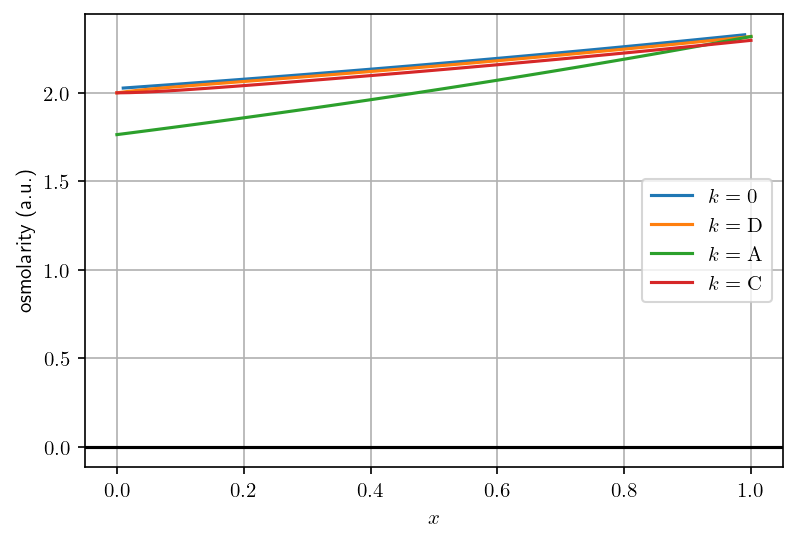
\includegraphics[width=\linewidth]{../results/7-20-2023/osm_low_solute_perm.png}
        \caption{$\gamma_u = \gamma_s = 0.1$}
        \label{fig:low_sol_perm}
        \vspace*{4mm}
    \end{subfigure}

    \begin{subfigure}{0.8\textwidth}
        \centering
        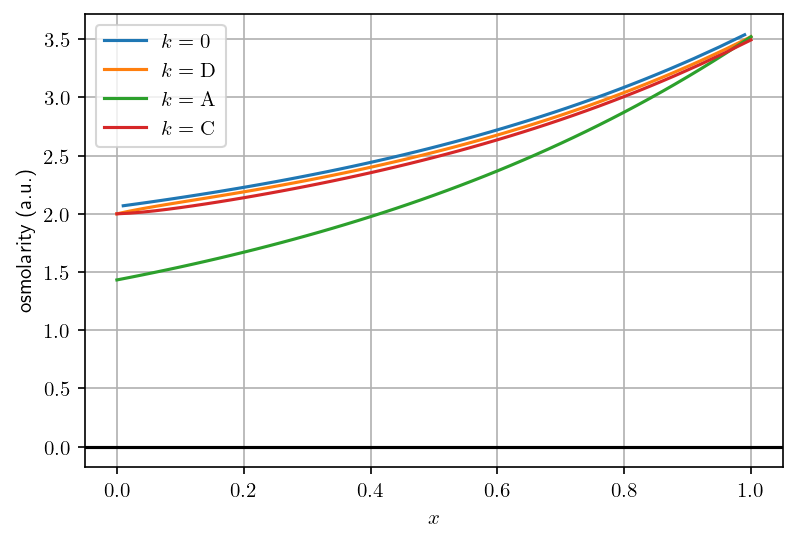
\includegraphics[width=\linewidth]{../results/7-20-2023/osm_high_solute_perm.png}
        \caption{$\gamma_u = \gamma_s = 1.2$}
        \label{fig:high_sol_perm}
    \end{subfigure}
    \caption{$\zeta_\mathrm{D} = \zeta_\mathrm{C} = 10$, $S = 1$, $U = 2$, $C = 2$}
    \label{fig:typical_sol}
\end{figure}

We can also see that the concentration gradient is increased when the solute permeability is higher (Figure \ref{fig:high_sol_perm}).
This is not so surprising; the more solute reabsorption, the more osmotic drive to concentrate the urine.
To understand the distinct roles between that of salt and urea, we plot the osmolarity at the papillary end as a function of solute permeabilities (Figure \ref{fig:pap_osm}).
We see that, as $\gamma_u$ vanishes, the osmolarity at the papillary end of each compartment becomes closer to the osmolarity at the inner-outer medullary junction.
Under such a condition, increasing the ascending tubule salt permeability has very little effect to the concentration gradient.
Therefore, urea is an `enabler' of salt reabsorption, while both salt and urea act as sources of osmotic drive.
\begin{figure}
    \centering
    \begin{subfigure}{0.5\textwidth}
        \centering
        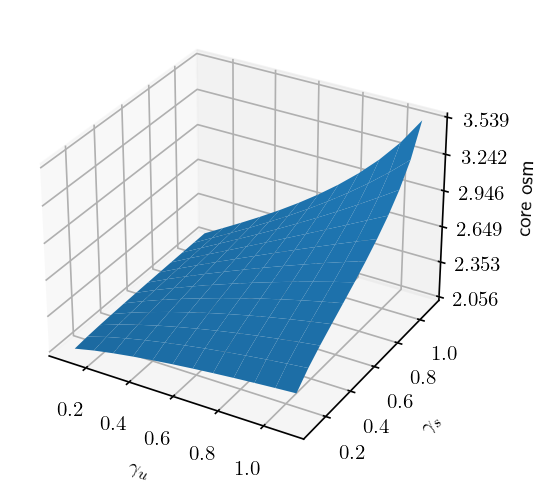
\includegraphics[width=\linewidth]{../results/7-20-2023/core_osm.png}
        \caption{papillary core osmolarity}
        \label{fig:core_osm}
    \end{subfigure}%
    \begin{subfigure}{0.5\textwidth}
        \centering
        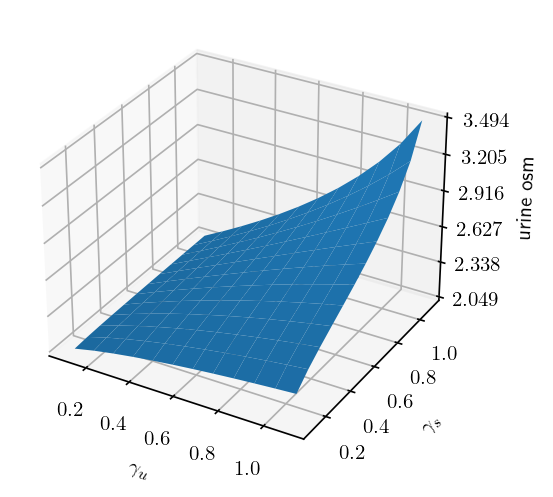
\includegraphics[width=\linewidth]{../results/7-20-2023/urine_osm.png}
        \caption{urine osmolarity}
        \label{fig:urine_osm}
    \end{subfigure}
    \begin{subfigure}{0.5\textwidth}
        \centering
        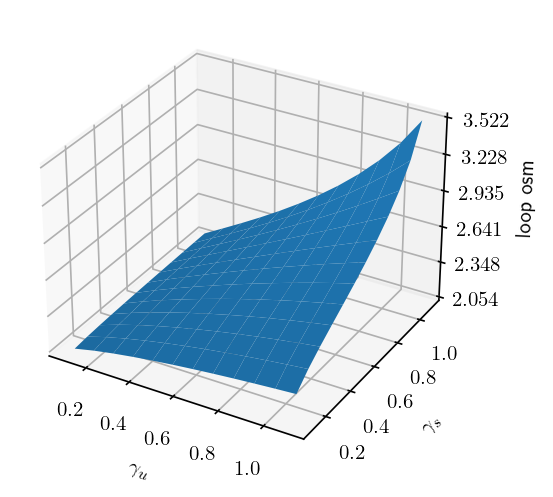
\includegraphics[width=\linewidth]{../results/7-20-2023/loop_osm.png}
        \caption{osmolarity at the turning of Henle's loop}
        \label{fig:loop_osm}
    \end{subfigure}
    \caption{$\zeta_\mathrm{D} = \zeta_\mathrm{C} = 10$, $S = 1$, $U = 2$, $C = 2$}
    \label{fig:pap_osm}
\end{figure}

There is yet another factor that can further enhance the effectiveness of the passive mechanism: the proportion of long-loop nephrons.
\begin{figure}
    \centering
    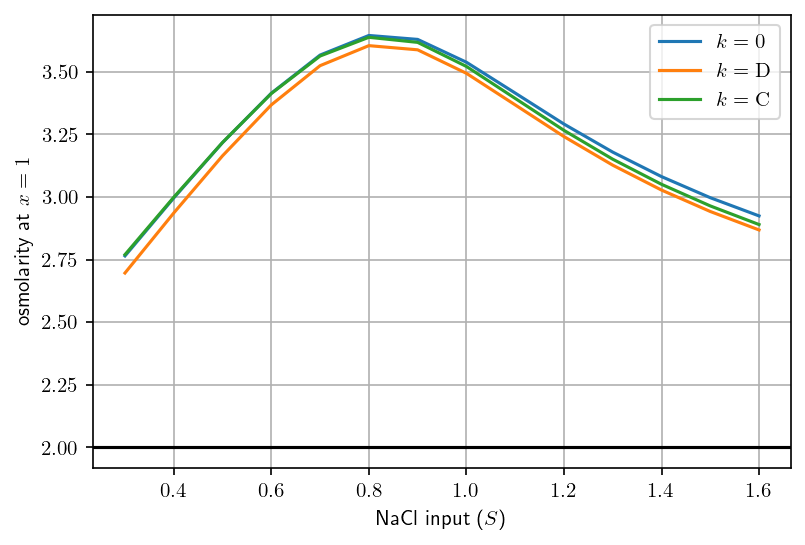
\includegraphics[width=0.8\textwidth]{../results/7-20-2023/osm_loop_fraction.png}
    \caption{$\zeta_\mathrm{D} = \zeta_\mathrm{C} = 10$, $\gamma_u = \gamma_s = 1.2$, $U = 2$, $C = 2$}
    \label{fig:loop_frac}
\end{figure}
The initial salt flux $S$ is proportional to the number of loops of nephron that descend pass the inner-outer medullary junction.
We see in the Figure \ref{fig:loop_frac} that the osmolarity at the papillary end is maximized at a certain value of $S$.
The rationale for this is that if there are less loops in the inner medulla, the salt load will not be enough to create a concentration gradient in the vascular core and the collecting tubule.
On the other hand, if there are too many loops, the water inside the descending tubule cannot be reabsorbed to the extent that heighten the salt concentration at the loop turning enough to effectively drive the salt reabsorption.

\end{document}